% Title Page

\backgroundsetup{%
    contents={%
        \begin{tikzpicture}
            %\pgfmathsetmacro{\myopacity}{mod(\thepage-1,4)*0.25+0.25}
            \node[opacity=0.35] {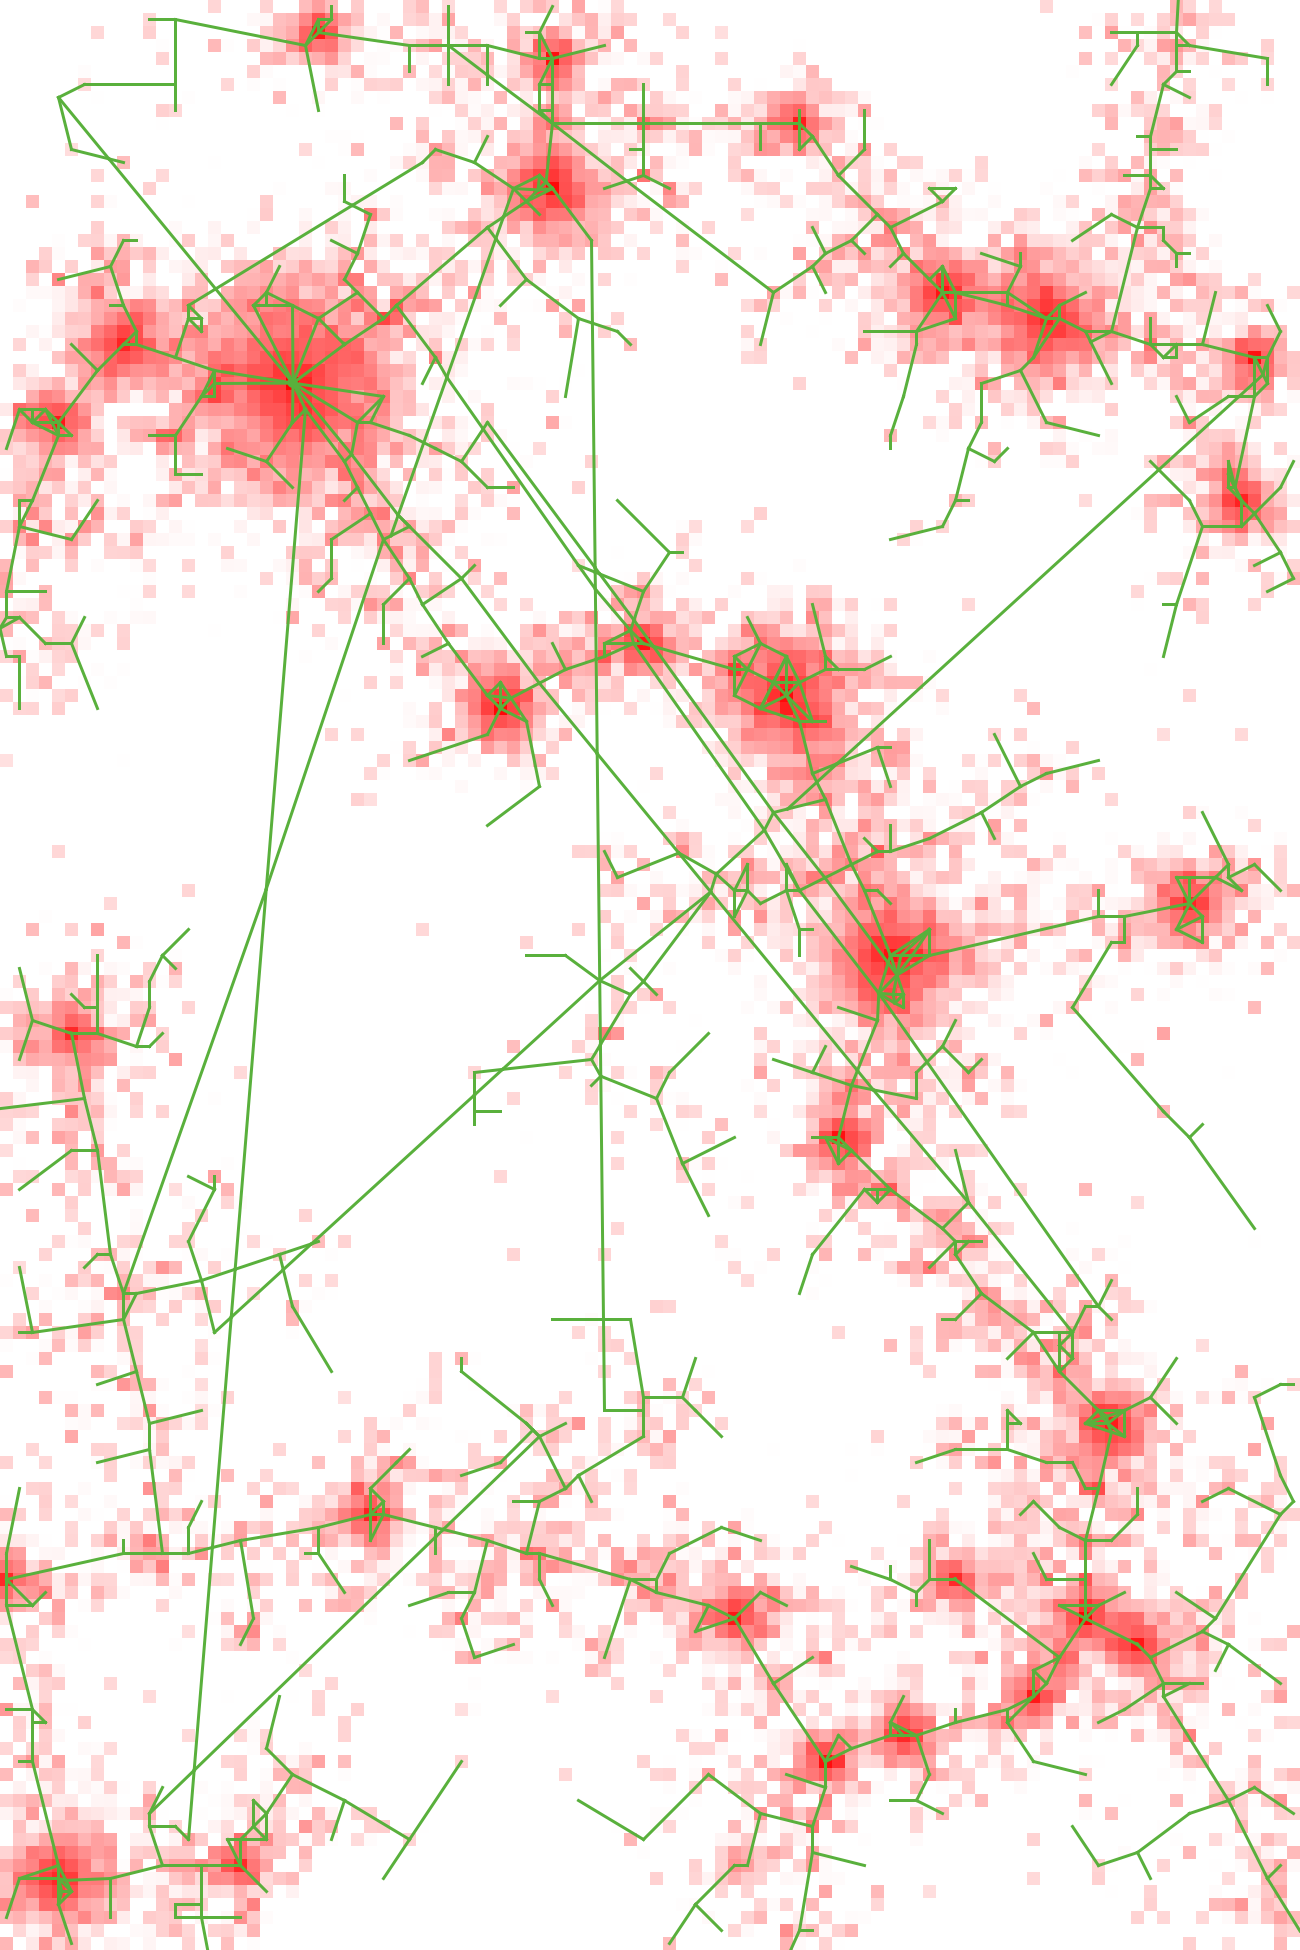
\includegraphics[width=\paperwidth]{Figures/Cover/cover2}};
        \end{tikzpicture}
    }
}


\begin{titlepage}

\begin{addmargin}[-1cm]{-3cm}
\begin{center}
\large

\hfill
\vfill

\begingroup
\spacedallcaps{Thèse de Doctorat}\\\medskip
\textit{pour obtenir le grade de}\\\medskip
\spacedallcaps{Docteur de l'Université Paris VII - Denis Diderot}\\\medskip
\textit{en }\\\medskip
\spacedallcaps{Géographie}\\\vspace{1cm}
\endgroup

\vfill

\begingroup
%\color{Maroon}
\textbf{\spacedallcaps{\myTitle}} \\ \bigskip % Thesis title
\endgroup

\vfill



% https://tex.stackexchange.com/questions/229593/gradient-to-transparent-horizontal-for-beamer-frametitle

%\vspace{-2cm}
%{\transparent{0.7} \includegraphics[width=\textwidth]{Figures/Cover/cover}} \\ %\vspace{0.5cm} % Picture
%\vspace{-3cm}

\textit{Présentée par}\\\medskip
\spacedlowsmallcaps{\myName}\\ % Your name
\bigskip


%\mySubtitle \\ \medskip % Thesis subtitle
%Under the supervision of \myProf and \myOtherProf \\ \medskip
Sous la direction de \myProf et \myOtherProf \\ \medskip
%\myDegree \\
\myDepartment \\  \medskip
%\myFaculty \\  \bigskip
%\myUni \\ \bigskip

\hspace{1.5cm}

\myTime\ -- \myVersion % Time and version

\hspace{1.5cm}

\textit{Composition du Jury :}

\medskip


\begin{adjustwidth*}{-0.5cm}{-2cm}
\begin{minipage}{0.28\linewidth}
\raggedright
\textbf{\noun{Arnaud Banos}}\\
\textbf{\noun{Florent Le Néchet}}\\
\textbf{\noun{Didier Josselin}}\\
\textbf{\noun{Catherine Morency}}
\end{minipage}
\begin{minipage}{0.7\linewidth}
\raggedright
Directeur de Recherche, CNRS (Directeur)\\
Maître de Conférence, Université Paris-Est (Directeur)\\
Directeur de Recherche, CNRS (Rapporteur)\\
Professeure, Ecole Polytechnique de Montréal (Rapporteuse)
\end{minipage}
\end{adjustwidth*}

\vfill

\end{center}
\end{addmargin}

\end{titlepage}


\backgroundsetup{%
    contents={}
}


